\documentclass[tikz,border=4pt]{standalone}
\usepackage[T1]{fontenc}
\usepackage[utf8]{inputenc}
\usepackage{amsmath,amssymb}
\usepackage{helvet}
\renewcommand{\familydefault}{\sfdefault}
\usepackage{pgfplots}
\pgfplotsset{compat=1.17}
\usetikzlibrary{arrows.meta,positioning,calc,fit,backgrounds,shapes.geometric}

\definecolor{cVis}{HTML}{1F77B4}
\definecolor{cTxt}{HTML}{D62728}
\definecolor{cProj}{HTML}{2CA02C}
\definecolor{cLLM}{HTML}{9467BD}
\definecolor{cConv}{HTML}{FF7F0E}
\definecolor{cAtt}{HTML}{17BECF}
\definecolor{cGray}{HTML}{7F7F7F}

\tikzset{
  blk/.style={draw, rounded corners=2pt, minimum height=8mm, align=center, font=\footnotesize, thick},
  tok/.style={draw, minimum size=3.2mm, inner sep=0pt},
  arr/.style={-{Stealth[length=2mm]}, thick},
}

\begin{document}
\begin{tikzpicture}[node distance=7mm]
  \node[blk, fill=cVis!15, minimum width=18mm, minimum height=14mm] (img) {Imagen\\$\mathbf{x}\in\mathbb{R}^{H\times W\times 3}$};
  \node[blk, fill=cVis!35, right=of img, minimum width=24mm, minimum height=14mm] (enc) {\textbf{Codificador}\\\textbf{de visión}\\(ViT, CNN, híbrido)};
  \node[right=6mm of enc] (vt) {\begin{tikzpicture}[scale=.9]\foreach \i in {0,...,5}{\node[tok,fill=cVis!40] at (\i*0.36,0) {};}\end{tikzpicture}};
  \node[below=0mm of vt, font=\scriptsize] {$N_v$ tokens visuales};
  \node[blk, fill=cProj!25, right=6mm of vt, minimum width=16mm, minimum height=14mm] (proj) {Proyector\\(MLP)};
  \node[blk, fill=cLLM!25, right=8mm of proj, minimum width=22mm, minimum height=22mm] (llm) {\textbf{LLM}\\decodificador\\autorregresivo};
  \node[above=8mm of proj, xshift=6mm] (tt) {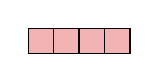
\begin{tikzpicture}[scale=.9]\foreach \i in {0,...,3}{\node[tok,fill=cTxt!35] at (\i*0.36,0) {};}\end{tikzpicture}};
  \node[above=0mm of tt, font=\scriptsize] {tokens de texto (pregunta)};
  \node[right=6mm of llm, font=\footnotesize, align=center] (out) {Respuesta\\en texto};
  \draw[arr] (img) -- (enc); \draw[arr] (enc) -- (vt); \draw[arr] (vt) -- (proj); \draw[arr] (proj) -- (llm);
  \draw[arr] (tt.east) -| ([xshift=-4mm]llm.north); \draw[arr] (llm) -- (out);
\end{tikzpicture}
\end{document}
